\documentclass[12pt,oneside]{book}
\newcommand{\TITLE}{Quantum Information Theory}
\usepackage[utf8]{inputenc}
\usepackage[margin=0.5in]{geometry}
\usepackage[usestackEOL]{stackengine}
\usepackage{amsmath , esint,braket,lmodern,mhchem,bohr,lewis,chemfig,draftwatermark,xcolor,graphicx , amssymb ,ragged2e , listings , siunitx , float , eqparbox, centernot , esvect , bm , fancyhdr , fourier-orns}
\usepackage[ddmmyyyy]{datetime}
\usepackage{fourier-orns}
\usepackage{changepage}
\usepackage{bbm}\usepackage{chngcntr}
\usepackage{hyperref}
\usepackage{ifthen}
\usepackage[many]{tcolorbox}
\DeclareMathOperator{\sech}{sech}
\DeclareMathOperator{\csch}{csch}
\DeclareMathOperator{\arcsec}{arcsec}
\DeclareMathOperator{\arccot}{arcCot}
\DeclareMathOperator{\arccsc}{arcCsc}
\DeclareMathOperator{\arccosh}{arcCosh}
\DeclareMathOperator{\arcsinh}{arcsinh}
\DeclareMathOperator{\arctanh}{arctanh}
\DeclareMathOperator{\arcsech}{arcsech}
\DeclareMathOperator{\arccsch}{arcCsch}
\DeclareMathOperator{\arccoth}{arcCoth} 
\DeclareMathOperator{\grad}{\vv{\text{grad}}} 
\DeclareMathOperator{\conj}{^*} 
\DeclareMathOperator{\vect}{vv} 
\DeclareMathOperator{\Vect}{\text{Vect}} 
\DeclareMathOperator{\degree}{c^\circ} 
\DeclareMathOperator{\degre}{^\circ} 
\DeclareMathOperator{\transpose}{^\dagger} 
\DeclareMathOperator{\adjoint}{^\dagger} 

\newcommand{\moyenne}[1]{\langle #1 \rangle} 
\newcommand{\lagrange}{\mathcal{L}}
\newcommand{\fourier}{\mathcal{F}}
\newcommand{\hilbert}{\mathcal{H}}
\newcommand{\p}{\mathcal{P}}
\newcommand{\x}{\chi}
\newcommand{\ve}[1]{\vv{#1}}
\newcommand{\push}[1]{\begin{adjustwidth}{5mm}{}#1\end{adjustwidth}}
\newcommand{\operator}[1]{\widehat{#1}}
\newcommand{\HRule}{\rule{\linewidth}{0.5mm}} % Defines a new command for the horizontal lines, change thickness here
\renewcommand{\chaptermark}[1]{\markboth{\MakeUppercase{#1}}{}}
\renewcommand{\headrule}{%
\vspace{-8pt}\hrulefill
\raisebox{-2.1pt}{\quad\decofourleft\decotwo\decofourright\quad}\hrulefill}
\definecolor{myred}{RGB}{255, 14, 0}
\everymath{\displaystyle}

\def\changemargin#1{\list{}{\leftmargin#1}\item[]}
\let\endchangemargin=\endlist 

\makeatletter
\newcommand*{\rom}[1]{\expandafter\@slowromancap\romannumeral #1@}%roman numbers
\makeatother

%hyperlink shit

\hypersetup{
    colorlinks,
    citecolor=black,
    filecolor=black,
    linkcolor=black,
    urlcolor=black
}
% Table specail cell , it's for making line break in table cell
\newcommand{\specialcell}[2][c]{%
  \begin{tabular}[#1]{@{}c@{}}#2\end{tabular}}

  \definecolor{main}{HTML}{5989cf}    % setting main color to be used
\definecolor{sub}{HTML}{cde4ff}     % setting sub color to be used

\tcbset{
    sharp corners,
    colback = white,
    before skip = 0.2cm,    % add extra space before the box
    after skip = 0.5cm      % add extra space after the box
}   
\newtcolorbox{boxH}{
    colback = sub, 
    colframe = main, 
    boxrule = 0pt, 
    leftrule = 6pt % left rule weight
}
\newtcolorbox{gpt}{
    sharpish corners, % better drop shadow
    boxrule = 0pt,
    toprule = 4.5pt, % top rule weight
    enhanced,
    fuzzy shadow = {0pt}{-2pt}{-0.5pt}{0.5pt}{black!35} % {xshift}{yshift}{offset}{step}{options} 
}
\definecolor{codegreen}{rgb}{0,0.6,0}
\definecolor{codegray}{rgb}{0.5,0.5,0.5}
\definecolor{codepurple}{rgb}{0.58,0,0.82}
\definecolor{backcolour}{rgb}{0.95,0.95,0.92}

\lstdefinestyle{mystyle}{
    backgroundcolor=\color{backcolour},   
    commentstyle=\color{codegreen},
    keywordstyle=\color{magenta},
    numberstyle=\tiny\color{codegray},
    stringstyle=\color{codepurple},
    basicstyle=\ttfamily\footnotesize,
    breakatwhitespace=false,         
    breaklines=true,                 
    captionpos=b,                    
    keepspaces=true,                 
    numbers=left,                    
    numbersep=5pt,                  
    showspaces=false,                
    showstringspaces=false,
    showtabs=false,                  
    tabsize=2,
    basicstyle = \small
}

\lstset{style=mystyle}
\SetWatermarkAngle{45} 
\SetWatermarkLightness{.99} 
\SetWatermarkFontSize{0.1cm} 
\SetWatermarkScale{0} 
\SetWatermarkText{supahaka}


\begin{document}
\pagestyle{fancy}
\fancyhf{}
\fancyfoot[R]{Tenji$_\text{org}$}
\fancyfoot[C]{\thepage}
\fancyfoot[L]{\tiny www.tenji.org}
\fancyhead[RO]{\nouppercase{\leftmark\hfill\TITLE}}


\DraftwatermarkOptions{stamp=false}
    \begin{titlepage}
        \begin{center}
            \vspace*{5cm}
            \Huge
            \HRule \\[0.4cm]
            \textbf{Project Tenji: \\ \TITLE}\\
            \Large 
            \HRule \\[1.5cm]
            \vspace{2cm}
            \vfill
        \end{center}
        \vfill
        { \scriptsize Project Tenji \copyright 2024 by Khalil Salahat and Mohamad El Moussawi  \\}
        { \scriptsize Hosted at tenji.org , contact : contact@tenji.org \\}
        { \scriptsize \NOTICEE  \\}
    \end{titlepage} 
    \tableofcontents
\DraftwatermarkOptions{stamp=true}
\chapter{INTRODUCTION}
\section{Classical Information}
The most basic piece of information is called a bit, and this basically represents a yes-no answer to a question.\\
To represent this \underline{mathematically} we use binary numbers,a binary number can be 0 or 1.\\
Physically we can implement a bit with an electrical circuit $\begin{cases}
        \text{ zero volts} \to \text{ binary 0}   \\
        \text{ + five volts} \to \text{ binary 1} \\
    \end{cases}$\\
The smallest number $n$ of bits required to represent $m$ different state :
\[ 2^n \geq m \]
$n$ bits can store $m$ different messages :
\[\log_2 (m) = n\]
A byte is a string of eight bits linked together ($\log_2 (256) = 8 $)
\section{Entropy and Shannon's information theory}
To get a more accurate estimation of the information content in a signal, the key step taken by Shannon was that he asked:\\
\begin{center}
    How likely is it that we are going to see a given piece of information?
\end{center}
And that allows us to characterize how much information we actually gain from a signal.\\
\begin{itemize}
    \item If a message has a very high probability of occurrence, then we don’t gain all that much new information when we come across it.
    \item On the other hand, if a message has a low probability of occurrence, when we are made of aware of it, we gain a significant amount of information.
\end{itemize}
Shannon quantified this by taking the base 2 logarithm of the probability of a given message occurring.\\
The information content of a message by I, and the probability of its occurrence by p, then :
\[I = -\log_2(p)\]
\begin{itemize}
    \item A message that is unlikely to occur has a low probability and therefore has a large information content.
    \item A message that is very likely to occur has a high probability and therefore has a small information content.
\end{itemize}
\underline{Example :}
\push{
    \scriptsize
    Let’s suppose that the probability of an earthquake not happening tomorrow is 0.995. The information content of this fact is \\
    $I = -\log_2(0.995) = 0.0072$.\\
    Now the probability that an earthquake does happen tomorrow is 0.005. The information content of this piece of information is \\
    $I' = -\log_2(0.005) = 7.7.6439$\\
}
Now let $X$ be a random variable characterized by a probability distribution $\vv{p}$, and suppose that it can assume one of the values $x_1,x_2,...,x_n$ with probabilities $p_1,p_2,...,p_n$\\
The Shannon entropy of $X$ is defined as :
\[H(X) = - \sum_ip_i\log_2(p_i)\]
\begin{itemize}
    \item If we are certain what the message is, the Shannon entropy is zero.
    \item The more uncertain we are as to what comes next, the higher the Shannon entropy.
\end{itemize}
\underline{Example :}
\push{
    \scriptsize
    Suppose that we have a signal that always transmits a “2”, The probability of obtaining a 2 is 1,\\
    So the entropy or disorder is : $H = -\log_2(1) = 0$\\
    A signal that has all the same characters with no changes has no disorder and hence no entropy.
}
\chapter{QUBITS AND QUANTUM STATES}
\section{The Qubit}
Qubit is the basic unit of information in quantum computing which is short for quantum bit.\\
A qubit can exist in the state $\ket{0},\ket{1}$ or also in a superposition state$\begin{cases}
        \ket{\psi} = \ket{0} \\
        \ket{\psi} = \ket{1} \\
        \ket{\psi} = \alpha\ket{0} + \beta\ket{1}
    \end{cases}$\\
Where $|\alpha|^2$ and $|\beta|^2$ tells us the probability of finding $\ket{\psi}$ in state $\ket{0}$ and $\ket{1}$.\\
$|\alpha|^2 + |\beta|^2 = 1$\\
$|\alpha|^2 = (\alpha)(\alpha\conj)$ and $|\beta|^2 = (\beta)(\beta\conj)$\\
When a qubit is measured, it is only going to be found to be in the state $\ket{0}$ or the state $\ket{1}$.\\
\section{Vector spaces}
A vector space $V$ is a nonempty set with elements $u, v$ called vectors for which the following two operations are defined:
\begin{itemize}
    \item Vector addition ,$w \in V, w =u +v$
    \item Scalar multiplication,$\alpha \in \mathbb{C}, \alpha u \in V $
\end{itemize}
in addition :
\begin{itemize}
    \item Associativity of addition : $(u+v) + w = u + (v+w)$
    \item zero vector such as : $u +0 = 0 + u  =u$
    \item additive inverse :$u +(-u) = (-u)+u=0$
    \item addition of vectors is commutative : $u + v = v +u$
\end{itemize}
One particular vector space that is important in quantum computation is the vector space is $\mathbb{C}$.\\
we label the elements of $\mathbb{C}$ by $\ket{a},\ket{b},\ket{c}$.\\
we write down a vector as column vector :
\[\ket{a} =  \left( \begin{matrix}
            a_1 \\
            a_2 \\
            ... \\
            a_n
        \end{matrix}\right)\]
Multiplication of a vector by a scalar proceeds as :
\[ \alpha \ket{a} = \alpha\left( \begin{matrix}
            a_1 \\
            a_2 \\
            ... \\
            a_n
        \end{matrix}\right) = \left( \begin{matrix}
            \alpha a_1 \\
            \alpha a_2 \\
            ...        \\
            \alpha a_n
        \end{matrix}\right) \]
Vector addition :
\[ \ket{a} + \ket{b} = \left( \begin{matrix}
            a_1 \\
            a_2 \\
            ... \\
            a_n
        \end{matrix}\right) + \left( \begin{matrix}
            b_1 \\
            b_2 \\
            ... \\
            b_n
        \end{matrix}\right) = \left( \begin{matrix}
            a_1 + b_1 \\
            a_2 + b_2 \\
            ...       \\
            a_n+b_n
        \end{matrix}\right)\]
\section{Linear combinations of vectors}
A linear combination of these vectors is given by
\[ \alpha_1\ket{v_1} + \alpha_2\ket{v_2} + ... + \alpha_n\ket{v_n} = \sum_{i=1}^n \alpha_i\ket{v_i} \]
An arbitrary qubit can be writes as $\ket{\psi} = \alpha\ket{0} + \beta\ket{1}$\\
$\ket{\psi} =  \left( \begin{matrix}
            \alpha \\
            \beta
        \end{matrix}\right) = \left( \begin{matrix}
            \alpha \\
            0
        \end{matrix}\right) + \left( \begin{matrix}
            0 \\
            \beta
        \end{matrix}\right) = \alpha \left( \begin{matrix}
            1 \\
            0
        \end{matrix}\right) + \beta\left( \begin{matrix}
            0 \\
            1
        \end{matrix}\right) \implies $ we identify $\ket{0} = \left( \begin{matrix}
            1 \\
            0
        \end{matrix}\right)$ and $\ket{1} = \left( \begin{matrix}
            0 \\
            1
        \end{matrix}\right)$

\subsubsection{Linear independence}
if one vector of the set can be written as a linear combination of the other vectors in the set, then the set is linearly dependent.\\
a set of vectors is that of linear independence if:
\[ \alpha_1\ket{v_1} + \alpha_2\ket{v_2} + ... + \alpha_n\ket{v_n} =0\]
\underline{Note that :}
\push{A spanning set of vectors for a given space V is not unique.}
\section{Basis and dimension}
When a set of vectors is linearly independent and they span the space, the set is known as \underline{a basis}.\\
We can express any vector in the space $V$ in terms of a linear expansion on a basis set.\\
The \underline{dimension} of a vector space $V$ is equal to the number of elements in the basis set.\\
A quantum state $\ket{\psi}$ can be written as a linear combination of a basis set $\ket{v_i}$ with complex coefficients of expansion $c_i$ as  :
\[\ket{\psi} = \sum_{i=1}^{n}c_i\ket{v_i} = c_1\ket{v_1} + c_2\ket{v_2} + ...+ c_n\ket{v_n} \]
The modulus squared of a given coefficient $c_i$ gives the probability that measurement finds the system in the state $\ket{v_i}$.
\section{Inner Products}
We write the inner product between two vectors $\ket{u},\ket{v}$ with the notation $\braket{u|v}$.\\

The inner product is a complex number, the conjugate of this complex number satisfies : $\braket{u|v}\conj = \braket{v|u}$.\\
The norm of a vector $u$ is : $||u|| = \sqrt{\braket{u|u}}$.\\
$\ket{u}\adjoint = \bra{u} \to \left( \begin{matrix}
            a_1 \\
            a_2 \\
            ... \\
            a_n
        \end{matrix}\right)\adjoint = (a_1\conj a_2\conj ... a_3\conj)$
\section{Orthonormality}
We say that $\ket{u},\ket{v}$ are orthogonal when
\[\braket{u|v} = 0\]
When the norm of a vector is unity, we say that vector is normalized
\[\braket{a|a} = 1\]
If each element of a set of vectors is normalized and the elements are orthogonal with respect to each other, we say the set is orthonormal.
\subsection{GRAM-SCHMIDT orthogonalisation}
An orthonormal basis can be produced from an arbitrary basis by application of the Gram-Schmidt orthogonalisation process.\\
let $\{ \ket{v_1},\ket{v_2},...,\ket{v_n} \}$,be a basis for an inner product space $V$.\\
The Gram-Schmidt process constructs an orthogonal basis $\ket{w_i}$ as follows :\\
$\ket{w_1} = \ket{v_1}$\\
$\ket{w_2} = \ket{v_2} - \frac{\braket{w_1|v_2}}{\braket{w_1|w_1}}\ket{w_1}$\\
....\\
$\ket{w_n} = \ket{v_n} - \frac{\braket{w_1|v_n}}{\braket{w_1|w_1}}\ket{w_1} - \frac{\braket{w_2|v_n}}{\braket{w_2|w_2}}\ket{w_2} - ... - \frac{\braket{w_{n-1}|v_n}}{\braket{w_{n-1}|w_{n-1}}}\ket{w_{n-1}}$\\
To form an orthonormal set using the Gram-Schmidt procedure, divide each vector by its norm.
\section{The Cauchy-Schwartz and triangle inequalities}
The Cauchy-Schwarz inequality :
\[ |\braket{\psi|\phi}|^2 \leq \braket{\psi|\psi}\braket{\phi|\phi} \]
The triangle inequality :
\[ \sqrt{\braket{\psi + \phi|\psi+\phi}} \leq \sqrt{\braket{\psi|\psi}} + \sqrt{\braket{\phi|\phi}} \]
\chapter{MATRICES AND OPERATORS}
An operator is a mathematical rule that can be applied to a function to transform it into another function.\\
An operator $\hat{A}$ is a mathematical rule that transforms a ket $\ket{\psi}$ into another ket that we will call $\ket{\phi}$:
\[\hat{A}\ket{\psi} = \ket{\phi}\]
Operators can act also on bras:
\[ \hat{A}\bra{\mu} = \bra{\nu} \]
We say that an operator is linear if :
\[\hat{A} (\alpha\ket{\psi_1}+\beta\ket{\psi_2}) = \alpha\hat{A}\ket{\psi_1} + \beta\hat{A}\ket{\psi_2}\]
The simplest operator is the identity operator $\hat{I}$ :
\[\hat{I} \ket{\psi} = \ket{\psi}\]
The zero operator :
\[\hat{0}\ket{\psi} = 0\]
\section{Outer Products}
The product of a ket $\ket{\psi}$ with a bra $\bra{\phi}$ which is written as $\ket{\psi}\bra{\phi}$, \underline{this quantity is an operator}.
\[(\ket{\psi}\bra{\phi})\ket{\xi} = \ket{\psi}\braket{\phi|\xi} = (\braket{\phi|\phi|\xi})\ket{\psi} \]
\section{The closure relation}
\[\sum_{i=1}^n \ket{u_i}\bra{u_i} = \hat{I}\]
The closure relation is often useful in manipulating expressions.\\
For example if $\braket{u_i|\psi} = c_i$, an arbitrary state $\ket{\psi}$ can be expanded in terms of the basis $\{ \ket{u_i} \}$ :
\[\ket{\psi}  = \hat{I}\ket{\psi} = \left( \sum_{i=1}^n\ket{u_i}\bra{u_i} \right)\ket{\psi} = \sum_{i=1}^{n}\ket{u_i}\braket{u_i|\psi} = \sum_{i=1}^nc_i\ket{u_i} \]
\section{Representations of operators using matrices}
We can find the matrix elements of the operator using the closure relation :
\[\hat{A} = \hat{I}\hat{A}\hat{I} = \left( \sum_i\ket{u_i}\bra{u_i} \right) \hat{A} \left( \sum_j \ket{u_j}\bra{u_j} \right) = \sum_{i,j}\braket{u_i|\hat{A}|u_j}\ket{u_i}\bra{u_j} \]
\[ \hat{A} =  \left( \begin{matrix}
            \braket{u_1|\hat{A}|u_1} & \braket{u_1|\hat{A}|u_2} & ...    & \braket{u_1|\hat{A}|u_n} \\
            \braket{u_2|\hat{A}|u_1} & \braket{u_2|\hat{A}|u_2} & ...    & \braket{u_2|\hat{A}|u_n} \\
                                     &                          & \ddots &                          \\
                                     &                          &        & \braket{u_n|\hat{A}|u_n} \\
        \end{matrix}\right) \]
When the matrix representation of an operator is given, it is written with respect to a certain basis.\\
in general :\[ \braket{u_i|\hat{A}|u_j} \not = \braket{\nu_i|\hat{A}|\nu_j} \]
\section{Hermitian,Unitary, and Normal operators}
An operator A is said to be normal if
\[ AA\adjoint = A\adjoint A \]
An operator A is said to be unitary if
\[UU\adjoint = U\adjoint U = I\]
An operator $\hat{A}$ is said to be Hermitian if
\[ \hat{A} = \hat{A}\adjoint \]
\section{Observables}
Observables are things we measure in order to characterize the quantum state of a particle
\subsection{The Pauli operators}
\begin{itemize}
    \item $\sigma_0\ket{0} = \ket{0} , \sigma_0\ket{1} = \ket{1}$
          \[\sigma_0 = \hat{I} = \left( \begin{matrix}
                      1 & 0 \\
                      0 & 1
                  \end{matrix}\right)\]
    \item $\sigma_1\ket{0} = \ket{1} , \sigma_1\ket{1} = \ket{0}$
          \[\sigma_1 = X = \left( \begin{matrix}
                      0 & 1 \\
                      1 & 0
                  \end{matrix}\right)\]
    \item $\sigma_2\ket{0} = -i\ket{1} , \sigma_2\ket{1} = i\ket{0}$
          \[\sigma_2 = Y = \left( \begin{matrix}
                      0 & -i \\
                      i & 0
                  \end{matrix}\right)\]
    \item $\sigma_3\ket{0} = \ket{0} , \sigma_3\ket{1} = -\ket{1}$
          \[\sigma_3 = Z = \left( \begin{matrix}
                      1 & 0  \\
                      0 & -1
                  \end{matrix}\right)\]
\end{itemize}
\section{Eigenvalues and Eigenvectors}
A given vector is said to be an eigenvector of an operator A if the following equation is satisfied
\[A\ket{\psi} = \lambda\ket{\psi}\]
The number $\lambda$ is called an eigenvalue of the operator A.\\
A common problem in quantum mechanics is the following: \\
given an operator, find its eigenvalues and eigenvectors.\\
The first step in this process is to find the eigenvalues using what is known as the characteristic equation :
\[\det|A-\lambda I| = 0\]
\section{Spectral Decomposition}
An operator A belonging to some vector space that is normal and has a diagonal matrix representation with respect to some basis of that vector space.\\
$\hat{A}$ satisfies the spectral decomposition for the basis $\ket{u_i}$ :
\[ A = \sum_{i=1}^n a_i\ket{u_i}\bra{u_i} \]
Where $a_i$ are the eigenvalues.
\section{The trace of an operator}
The trace of the operator is the sum of the diagonal elements.
\[ Tr(A) = \sum_{i=1}^n\braket{u_i|A|u_i} \]
\subsubsection{Proprieties}
\begin{itemize}
    \item The trace is cyclic,$Tr(ABC) = Tr(CAB) = Tr(BCA)$
    \item The trace of an outer product is the inner product
          \[Tr(\ket{\phi}\bra{\psi}) = \braket{\psi|\phi}\]
          \[Tr(A\ket{\psi}\bra{\phi}) = \braket{\psi|A|\phi}\]
    \item The trace is basis independent.\\
          let $\ket{u_i}$ and $\ket{\nu_i}$ be two bases for some Hilbert space,then $Tr(A) = \sum\braket{u_i|A|u_i} = \sum\braket{\nu_i|A|\nu_i}$
    \item The trace of an operator is equal to the sum of its eigenvalues.
    \item The trace is linear
          \[Tr(\alpha A) = \alpha Tr(A),Tr(A+B) = Tr(A) + Tr(B)\]
\end{itemize}
\section{The expectation value of an operator}
The expectation value of an operator is the mean or average value of that operator with respect to a given quantum state.\\
if a quantum state $\ket{\psi}$ is prepared many times, and we measure a given operator $A$ each time , the average of measurement result is the expectation value
\[\moyenne{A} = \braket{\psi|A|\psi} \]
\section{Function of operators}
The function of an operator can be found by calculating its Taylor expansion :
\[ f(A) = \sum_{n=0}^\infty a_n A^n \]
If an operator $A$ is normal and has a spectral expansion given by $A = \sum_i a_i\ket{u_i}\bra{u_i}$ then
\[f(A) = \sum_i f(a_i)\ket{u_i}\bra{u_i}\]
\section{Unitary transformation}
A method known as a unitary transformation can be used to transform the matrix representation of an operator in one basis to a representation of that operator in another basis.\\
The change of basis matrix from a basis $\ket{u_i}$ to a basis $\ket{v_i}$ is given by :
\[ U = \left( \begin{matrix}
            \braket{\nu_1|u_1} & \braket{\nu_1|u_2} \\
            \braket{\nu_2|u_1} & \braket{\nu_2|u_2}
        \end{matrix}\right) \]
We write a state vector $\ket{\psi}$ given in the $\ket{u_i}$ basis in terms of the new $\ket{\nu_i}$ basis as
\[ \ket{\psi'} = U\ket{\psi} \]
\section{Projection operators}
A projection operator is an operator that can be formed by writing the outer product using a single ket
\[P = \ket{\psi}\bra{\psi}\]
A projection operator is hermitian.\\
if the state $\ket{\psi}$ is normalized then a projection operator is equal to its own square :
\[P^2 = P\]
\section{Commutator}
The commutator of two operators A and B is defined as :
\[ [A,B] = AB - BA \]
When $ [A,B] = 0 $, we say that the operators A and B commute.\\
The commutator is antisymmetric :
\[ [A,B] = -[B,A] \]
The commutator is linear :
\[ [A,B+C] = [A,B] + [A,C] \]
We can use the following rule of distributivity :
\[ [A,BC] = [A,B]C + B[A,C] \]
\section{Uncertainty}
The uncertainty $\Delta A$,is a statistical measure of the spread of measurements about the mean
\[\Delta A = \sqrt{\moyenne{A^2} - \moyenne{A}^2} \]
Two operators A and B, it can be shown that the product of their uncertainties satisfies
\[\Delta A\Delta B \geq \frac{1}{2} | \moyenne{[A,B]} | \]
This is a generalization of the famous \underline{Heisenberg uncertainty principle}
\section{Singular Value Decomposition (SVD)}
Every $m\times n$ matrix factors into
\[A = U\Sigma V^T\]
Where $\begin{cases}
        U  \text{ is } m\times m \text{ orthogonal matrix}   \\
        \Sigma \text{ is } m\times n \text{ diagonal matrix} \\
        V^T \text{ is } n\times n \text{ orthogonal matrix }
    \end{cases}$
\[ A =  \left( \begin{matrix}
            u_1 & u_2 \\
        \end{matrix}\right) \left( \begin{matrix}
            \sigma_1 & 0        \\
            0        & \sigma_2 \\
        \end{matrix}\right) \left( \begin{matrix}
            v_1^T \\
            v_2^T \\
        \end{matrix}\right)\]
$\begin{cases}
        \sigma \text{ Are the singular values }  \\
        v \text{ Are the right singular vectors} \\
        u \text{ Are the left singular vectors }
    \end{cases}$
\subsubsection{What are $ U ,\Sigma$ and $V$}
$A^TA = (V\Sigma^TU^T)U\Sigma V^T = V\Sigma^T\Sigma V^T$ , $\Sigma^T\Sigma$ is a diagonal matrix.\\
By the usual diagonalisation the eigenvalue $\lambda$ for the matrix $A^TA$ are in $\Sigma^T\Sigma$ and the eigenvectors are in $V$ .\\
Then $\lambda$ for $A^TA$ are the singular value squared $\sigma^2$ for $A$.\\
Now we have $\Sigma $ and $V$ how we get hold of $U$\\
$AA^T = U\Sigma V^T V \Sigma^T U^T = U\Sigma\Sigma^T U^T $\\
So $U $ is eigenvector matrix for $AA^T$ ,$AA^T $ and $A^TA$ have the same eigenvalues\\


{\scriptsize{Refference : MIT RES.18-009 Learn Differential Equations: Up Close with Gilbert Strang and Cleve Moler, Fall 2015}}
\pagebreak
\section{THE POSTULATES OF QUANTUM MECHANICS}
\subsection{Postulate 1 : The state of a System}
\begin{itemize}
    \item The state of a quantum system is a vector $\ket{\psi(t)}$ in a Hilbert space.
    \item The state $\ket{\psi(t)}$ contains all information that we can obtain about hte system.
    \item We work with normalized states such that $\braket{\psi|\psi} =1$.
\end{itemize}
\subsection{Postulate 2: Observable quantities represented by operators}
\begin{itemize}
    \item To every dynamical variable $A$ that is a physically measurable quantity, there corresponds an operator $A$.
    \item The operator $A$ is Hermitian and its eigenvectors form a complete orthonormal basis of the vector space.
\end{itemize}
\subsection{Postulate 3: Measurements}
\begin{itemize}
    \item The possible results of measurement of a dynamical variable $A$ are the eigenvalues $a_n$ of the operator $A$ corresponding to that variable.
    \item $A = \sum_n a_n P_n$ where $P_n$ is the projection operators $P_n = \ket{u_n}\bra{u_n}$, The probability of obtaining measurement result $a_n$ is given by :
          \[ Pr(a_n) = \braket{\psi|P_n|\psi}  \]
    \item The probability amplitude $c_n = \braket{u_n|\psi}$ gives us the probability of obtaining measurement result $a_n$ as
          \[ Pr(a_n) = \frac{|\braket{u_n|\psi} |^2}{\braket{\psi|\psi}} = \frac{|c_n|^2}{\braket{\psi|\psi}} \]
    \item A measurement result $a_n$ causes the collapse of the wave-function,meaning that the system is left in state $\ket{u_n}$
\end{itemize}
\subsection{Postulate 4: Time evolution of the system}
\begin{itemize}
    \item The time evolution oa a closed quantum system is governed by the Schrodinger equation:
          \[ i\hbar \frac{\partial}{\partial t}\ket{\psi} = H\ket{\psi} \]
          Where $H$ is the Hamiltonian
    \item The state of the system at a later time $t$ is given by
          \[ \ket{\psi(t)} = e^{-i\frac{Ht}{\hbar}}\ket{\psi(0)} \]
          Therefore the time evolution of a quantum state is governed by the unitary operator
          \[ U = e^{-i\frac{Ht}{\hbar}} \]
\end{itemize}

\chapter{TENSOR PRODUCTS}
In the context of quantum information processing, it is necessary to work with multi particles states.\\
Suppose that $H_1$ and $H_2$ are two Hilbert spaces of dimension $N_1$ and $N_2$.\\
We can put these two Hilbert spaces together to construct a larger Hilbert space $H$
\[ H = H_1 \otimes H_2  \]
The dimension of $H$ : $ \text{dim}(H) = N_1N_2$\\\\
Let $\ket{\phi} \in H_1$ and $\ket{\xi} \in H_2 $, we can construct a vector $\ket{\psi} \in H$ :
\[\ket{\psi} = \ket{\phi} \otimes\ket{\xi}\]

\begin{itemize}
    \item The tensor product of two vectors is linear.
          \[\ket{\phi} \otimes [ \ket{\xi_1} + \ket{\xi_2} ] = \ket{\phi} \otimes \ket{\xi_1} + \ket{\phi} \otimes \ket{\xi_2}\]
          \[ [\ket{\phi_1} +\ket{\phi_2} ]\otimes \ket{\xi} = \ket{\phi_1}\otimes\ket{\xi} + \ket{\phi_2}\otimes\ket{\xi} \]
    \item Tensor product is linear with respect to scalars
          \[ \ket{\phi} \otimes (\alpha\ket{\xi}) = \alpha\ket{\phi} \otimes \ket{\xi} \]
    \item The order of the tensor product is not relevant
          \[ \ket{\phi} \otimes \ket{\xi} = \ket{\xi} \otimes \ket{\phi} \]
\end{itemize}
\section{Inner product}
Suppose $ \begin{cases}
        \ket{\psi_1} = \ket{\phi_1} \otimes\ket{\xi_1} \\
        \ket{\psi_2} = \ket{\phi_2} \otimes \ket{\xi_2}
    \end{cases}$
\[ \braket{\psi_1|\psi_2} =  ( \bra{\phi_1}\bra{\xi_1} )(\ket{\phi_2}\ket{\xi_{2}}) = \braket{\phi_1|\phi_2}\braket{\xi_1|\xi_2} \]
\section{Matrix Representation}
\[ \ket{\phi} =  \left( \begin{matrix}
            a \\
            b
        \end{matrix}\right) \text{ and } \ket{\xi} = \left( \begin{matrix}
            c \\
            d
        \end{matrix}\right) \]
The tensor product :
\[ \ket{\phi} \otimes  \ket{\xi} =
    \left( \begin{matrix}
            a \\
            b
        \end{matrix}\right) \otimes \left( \begin{matrix}
            c \\
            d
        \end{matrix}\right) =  \left( \begin{matrix}
            ac \\
            ad \\
            bc \\
            bd
        \end{matrix}\right)
\]
\section{Operators and tensor product}
Let $A$ be an operator that acts on vectors $\ket{\phi}$, and B act on vectors $\ket{\xi}$
\[ (A\otimes B)\ket{\psi} = (A\otimes B)(\ket{\phi}\otimes\ket{\xi})=(A\ket{\phi})\otimes(B\ket{\xi}) \]
\section{Tensor Products of matrices}
Let
\[ A =  \left( \begin{matrix}
            a_{11} & a_{12} \\
            a_{21} & a_{22} \\
        \end{matrix}\right) , B = \left( \begin{matrix}
            b_{11} & b_{12} \\
            b_{21} & b_{22} \\
        \end{matrix}\right)\]
The matrix representation of the tensor product $A\otimes B$ is
\[ A\otimes B =  \left( \begin{matrix}
            a_{11}B & a_{12}B \\
            a_{21}B & a_{22}B \\
        \end{matrix}\right) =  \left( \begin{matrix}
            a_{11}b_{11} & a_{11}b_{12} & a_{12}b_{11} & a_{12}b_{12} \\
            a_{11}b_{21} & a_{11}b_{22} & a_{12}b_{21} & a_{12}b_{22} \\
            a_{21}b_{11} & a_{21}b_{12} & a_{22}b_{11} & a_{22}b_{12} \\
            a_{21}b_{21} & a_{21}b_{22} & a_{22}b_{21} & a_{22}b_{22}
        \end{matrix}\right)  \]
\section{Note}
Not all states can be written as product of states, this is what will be called later entanglement.

\chapter{THE DENSITY OPERATOR}
\section{The density operator for a pure state}
When a system is in a definite state, we say the system is in a pure state.\\
The density operator is an average operator that will allow us to describe a statistical mixture.\\
The density operator for a state $\ket{\psi}$ is given by :
\[ \rho = \ket{\psi}\bra{\psi} =  \left( \begin{matrix}
 a_1 \\ 
 a_2 \\ 
 \vdots 
\end{matrix}\right)  \left( \begin{matrix}
 a_1\conj&a_2\conj  &\hdots  \\ 
\end{matrix}\right) =  \left( \begin{matrix}
 |a_1|^2&a_1a_2\conj  & \hdots  \\ 
 a_2a_1\conj&|a_2|^2  & \hdots  \\ 
&  & \ddots
\end{matrix}\right) \]
Then, diagonal elements are probabilities of being in the state $\ket{u_i} :$
\[p_i = |a_i|^2 = \braket{u_i|\psi}\braket{\psi|u_i} = \braket{u_i|\rho|u_i}\]

Due to the conservation of probability the trace of the density operator is always 1
\[Tr(\rho) = \sum_j\braket{u_j|\rho|u_j} = \sum_j\braket{u_j|\psi}\braket{\psi|u_j} =\sum_jc_jc_j\conj = \sum_j|c_j|^2 = 1\]
\subsection{Properties of a density operator}
\begin{itemize}
    \item The density operator is Hermitian
    \item $Tr(\rho) =1$
    \item $\rho$ is a positive operator, meaning $\braket{u|\rho|u} \geq 0$ for any state vector $\ket{u}$
\end{itemize}
If a system is in a pure state $\ket{\psi}$ then :
\[\rho^2 = \rho\]
\[ Tr(\rho^2) =1 \]
\section{Using the density operator to find the expectation value}
The expectation value of an operator $A$ can be written in terms of the density operator as:
\begin{align*}
    \moyenne{A} & = \sum_{k,l = 1}^n \braket{u_l|\rho|u_k}\braket{u_k|A|u_l}              \\
                & = \sum_{l=1}^n\braket{u_l|\rho ( \sum_{k=1}^n \ket{u_k}\bra{u_k})A|u_l} \\
                & = \sum_{l=1}^n\braket{u_l|\rho A|u_l}                                   \\
                & = Tr(\rho A)
\end{align*}
\section{Time evolution}
\[ i\hbar\frac{d\rho}{dt} = [H,\rho] \]
For a closed system the time evolution of the density operator can also be written in terms of a unitary operator $U$\\
\[ \rho(t) = U\rho(t_0)U\adjoint \]
A pure state will always be a pure state if the system is “isolated” or closed.
\section{The density operator for a mixed state}
For a state $\ket{\psi_i}$,denote the probability that a member of the ensemble has been prepared in the state $\ket{\psi_i}$ as $p_i$,then the density operator for the entire system is :
\[ \rho = \sum_{i=1}^n p_i\rho_i = \sum^n_{i=1}p_i\ket{\psi_i}\bra{\psi_i} \]

\section{Probability of obtaining a given measurement result}
The probability of obtaining $a_n$ can be calculated using the density operator
\[ p(a_n) = \braket{u_n|\rho|u_n}\]
\section{Characterizing mixed states}
The coherence is the capability of different components of a state to interfere with one another.
\begin{itemize}
    \item A mixed state is a classical statistical mixture of two or more states.\\
          The state has no coherence.\\
          Therefore the off-diagonal terms of the density operator are zero.
    \item A pure state will have nonzero off-diagonal terms.
\end{itemize}
$Tr(\rho^2) =1 $ for a pure state .The same is not true in the case of mixed state.
\begin{itemize}
    \item $Tr(\rho^2) <1$ for a mixed state.
    \item $Tr(\rho^2) = 1$ for a pure state.
\end{itemize}
\section{Completely mixed states}
In a completely mixed state the probability for the system to be in each given state is identical.\\
In that case the density operator is a constant multiple of the identity matrix.\\
If the state space has $n$ dimensions, then
\[ \rho = \frac{1}{n}I \]
So for a completely mixed state we have
\[ Tr(\rho^2) = Tr(\frac{1}{n^2}I) = \frac{1}{n^2}Tr(I) = \frac{1}{n}  \]
\section{Bloch representation}
We can write any matrix as a linear combination of the sigma matrices. \\
Arbitrary density matrix : 
\[\rho = \frac{a_0 + \vv{a}.\vv{\sigma}}{2}\]
With $\begin{cases}
    a_x = Tr(\sigma_x\rho)\\
    a_y = Tr(\sigma_y\rho)\\
    a_z = Tr(\sigma_z\rho)
\end{cases}$
\begin{center}
    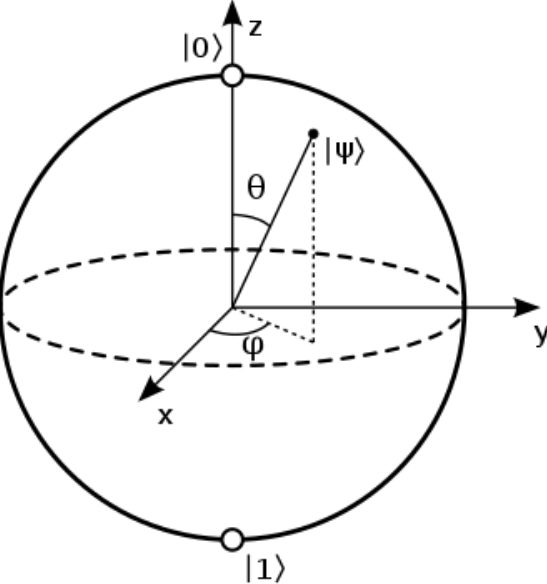
\includegraphics[width=0.2\linewidth]{../pic/3327/1.png}
\end{center}
% If we take $c_1$ real, $c_2$ will have a phase : $c_1 = \cos(\frac{\theta}{2});c_2 = e^{i\beta}\sin(\frac{\theta}{2})$
\section{Partial Trace}
    Given bipartite system in a state $\rho_{AB}$\\
    We can be interested in one of the two subsystems,we can then trace out the other one.\\
    Reduced density matrix :
    \[ \rho_A = Tr_B(\rho_{AB}) = \braket{0_B|\rho_{AB}|0_B} + \braket{1_B|\rho_{AB}|1_B} \]
    \[ \rho_B = Tr_A(\rho_{AB}) = \braket{0_A|\rho_{AB}|0_A} + \braket{1_A|\rho_{AB}|1_A} \]
    A reduced density matrix is that of a pure system if and only if the initial state is a pure and it is a product of states.
\chapter{QUANTUM MEASUREMENT THEORY}
\section{Distinguishing quantum states and measurement}
An act of measurement disturbs a quantum system in a fundamental way.\\
The measurement of a quantum system involves some type of interaction or coupling of that system with a measuring device.\\
That device can be thought of as part of the larger environment which the quantum system is a part of.\\

If the system is initially described by some density operator $\rho_0$,then the state of the system at time $t$ will be 
\[ \rho_t = U\rho_0U\adjoint \]
The dynamics of a quantum system is trace-preserving ($Tr(\rho_0) = Tr(\rho_t)$).\\
While time evolution is trace-preserving, measurement is described by trace-decreasing quantum operations.\\
A quantum operation involving measurement, described by a measurement operator that we will denote by $M_m$, transforms a density operator $\rho$ according to $\rho' = M_m\rho M_m\adjoint$.\\
In this case $Tr(\rho') \leq 1$

\section{Projective Measurements}
The idea of making a projective measurement is based on the following notion:
\begin{center}
    Given a set of mutually exclusive possible states, what state is the system is in?
\end{center}
\subsection{Properties}
    \begin{itemize}
        \item A projection operator $P$ is Hermitian and equal to its own square 
            \[P = P \adjoint , P^2 = P\]
        \item $P_1$ and $P_2$ orthogonal if 
            \[ P_1P_2\ket{\psi} = 0 \]
        \item  A complete set of orthogonal projection operators is one 
            \[ \sum_i P_i = I \]
        \item The number of projection operators is determined by the dimension of the Hilbert space that describes the system.\\
        If the dimension of the Hilbert space is $d$ and there are $m$ projection operators
        \[ m\leq d \]
        \item If two projection operators commute, then their product is also a projection operator.
        \item The probability of finding the ith outcome when a measurement is made is
            \[ Pr(i) = |P_i\ket{\psi}|^2 = (P_i\ket{\psi})\adjoint(P_i\ket{\psi}) = \braket{\psi|P_i^2|\psi} = \braket{\psi|P_i|\psi} \]
        \item The probability of obtaining measurement result $a_i$ can be written as 
            \[ Pr(i) = \braket{\psi|P_i|\psi} = Tr(P_i\ket{\psi}\bra{\psi}) \]
    \end{itemize}
\subsection{Collapse of the wave function}
while the state of the system prior to measurement could be a superposition of basis states after measurement the system collapses to the basis state that corresponds to the measurement result that was obtained.
\[ \ket{\psi'} = \frac{P_i\ket{\psi}}{\sqrt{ \braket{\psi|P_i|\psi}}} \]
\section{Generalized measurements}
    We denote a measurement operator by $M_m$, he probability that we find measurement result $m$ is
    \[ Pr(m) \braket{ \psi|M_m\adjoint M_m|\psi } \]
    After a measurement the state of the system is 
    \[ \ket{\psi'} = \frac{M_m\ket{\psi}}{\sqrt{\braket{\psi|M_m\adjoint M_m|\psi}}} \]
    Measurements when a system is described by a density operator.\\
    If a quantum system is described by a density operator $\rho$ , the probability of finding measurement result $m$ is 
    \[ Pr(m) = Tr(M_m\adjoint M_m \rho) \]
    If the measurement is described by a set of orthogonal projection operators $P_i = \ket{u_i}\bra{u_i}$ corresponding to measurement result $i$ then the probability of finding that measurement result is
    \[ Pr(i) = Tr(P_i\adjoint P_i \rho) = Tr(\ket{u_i}\bra{u_i}\rho) = \braket{u_i|\rho|u_i} \]

\section{Positive operator-valued measures}
Known as POVM, A POVM consists of a set of positive operators commonly denoted by $E_m$.\\
The probability of obtaining measurement result $m$ in this case is given by
\[Pr(m) = \braket{\psi|E_m|\psi}\]
The POVM allows us to construct a more general type of measurement operator to describe measurements where projective measurements do not apply in the real world.\\
A POVM  allows us to describe measurements on the system without regard to the post measurement state.

\chapter{ENTANGLEMENT}
One of the most unusual and fascinating aspects of quantum mechanics is the fact that particles or systems can become entangled.\\
For the simplest two quantum systems case we denote the systems $A$ and $B$.\\
If these systems are entangled, this means that the values of certain properties of system $A$ are correlated with the values that those properties will assume for system $B$.

When a system is entangled, this means that the individual component systems are really linked together as a single entity.\\
Any measurement that measures a part of the system is really a measurement on the entire system.\\

If two systems are entangled, the description of each system has to be made with reference to the state of the other system, even if the component systems are spatially separated and non interacting.
\section{BELL STATE}
They are known as the four maximally entangled two-qubit Bell states and they form a maximally entangled basis
\begin{itemize}
    \item $\ket{\beta_{00}} = \frac{\ket{00} + \ket{11}}{\sqrt{2}}$
    \item $\ket{\beta_{01}} = \frac{\ket{01} + \ket{10}}{\sqrt{2}}$
    \item $\ket{\beta_{10}} = \frac{\ket{00} - \ket{11}}{\sqrt{2}}$
    \item $\ket{\beta_{11}} = \frac{\ket{01} - \ket{10}}{\sqrt{2}}$
\end{itemize}
\section{When is a state entangled}
    Not all states $\ket{\psi} \in H_A \otimes H_B$ are entangled.\\
    When two systems are entangled, the state of each composite system can only be described with reference to the other state.\\
    If two states are not entangled, we say that they are a product state or separable.\\
    If $\ket{\psi} \in H_A$ and $\ket{\phi} \in H_B$ and $\ket{\xi} = \ket{\psi}\otimes\ket{\phi}$, then $\ket{\xi}$ is a product state
\section{Entanglement fidelity}
Consider a density operator for a single qubit that is diagonal with respect to the computational basis
\[ \rho = f\ket{0}\bra{0} + (1-f)\ket{1}\bra{1} \]
The parameter $f$ is known as the entanglement fidelity.

\chapter{Quantum noise and error correction}
In the treatment of quantum theory we’ve used so far we have been looking at closed systems.\\
These are quantum systems that do not interact with the outside world.That is, an idealized model.\\
In reality, quantum systems interact with the outside environment.\\
The problem if that interactions with the environment can introduce noise and cause errors.\\

We are going to have to develop a mathematical formalism to describe quantum systems that interact with the environment.\\
We refer to systems of this type as open systems.
\section{Single-Qubit errors}
    The ability to work with superposition states is what gives quantum computers their power.\\
    When a quantum system interacts with the environment  superposition can be lost,we call this process decoherence.\\
    Quantum noise acts on qubits via the application of one of the operators $I,X,Y,Z$.\\
    \subsection{Bit flip errors}
        We have $\ket{0} \to \ket{1}$ and $\ket{1} \to \ket{0}$\\
        This type of error is described by the X operator.
    \subsection{Phase flip errors}
        We have $\ket{x}\to (-1)^x\ket{x}$\\
        This type of error is described by the Z operator. \\

    The $Y$ operators is related to a phase flip followed by a bit flip
\section{Quantum operations and Krauss operators}
    The system density operator $\rho$.\\
    $\Phi(\rho)$ is a quantum operation,it is a mapping that describes the evolution of the system.\\
    The new system density operator $\rho'$
    \[\Phi(\rho) = \rho'\]
    Unitary evolution :$\Phi(\rho) = U\rho U\conj$\\
    Measurement : $\Phi(\rho) = M_m\rho M_m\conj$ \\

    If we have a set of operators $A_k$ that aren't necessarily unitary:
    \[ \Phi(\rho) = \sum_{k=1}^nA_k\rho A_k\conj \]
    The $A_k$, which are known as operation elements, cas satisfy a completeness relation 
    \[ \sum_{k=1}^n A_kA_k\conj = I \]

    To Calculate $A_k$ we define :
    \begin{itemize}
        \item $\rho$ is the density operator for the system.
        \item We denote the basis states of the environment by $\ket{e_k}$.
        \item $\ket{e_0}$ is the environment state
        \item $\sigma$ is the density operator for the environment.
    \end{itemize}
    \[ A_k = \braket{e_k|U|e_0} \]
\section{Some channels}
\subsection{Depolarization channel}
    Quantum noise is often described in terms of channels.\\
    The depolarization channel is known as when $p$  is a probability that the principal system evolves into a completely mixed state.\\
    and $(1-p)$ is the probability that the system stays the same.

    \[ \Phi(\rho) = (1-p)\rho + p\frac{1}{2}I \]
\subsection{Bit flip and phase flip channel}
    There is a probability $p$ that nothing happens to the qubit, While there is a probability $(1-p)$ that there is a bit flip error.
    \[ \Phi(\rho) = p\rho+(1-p)X\rho X \]
    There is a probability $p$ that nothing happens to the qubit, while there is a probability $(1-p)$ that there is a phase flip error.
    \[ \Phi(\rho) = p\rho + (1-p)Z\rho Z \]
\section{Amplitude damping}	
Real physical systems lose energy. When describing a quantum system undergoing energy dissipation because of some type of interaction with the environment, we apply a quantum operation known as amplitude damping.
\section{Phase damping}
Phase damping is a quantum process that involves information loss, but unlike amplitude damping, it does not involve energy loss. Specifically phase damping involves the loss of information about relative phases in a quantum state.


    

\chapter{TOOLS OF QIT}
\section{The no-Cloning theorem}
The remarkable power of a quantum computer comes from the fact a qubit can exist in a superposition.\\
Given this fact, can we make an exact copy of an arbitrary qubit?\\
It turns out the answer is no\\
\underline{Proof :}\\
Consider two pure states $\ket{\psi}$ and $\ket{\phi}$, and suppose that there exists a unitary operator $U$ such that 
\[ U(\ket{\psi}\otimes\ket{\xi}) = \ket{\psi} \otimes\ket{\psi} \]
%{\tiny i guess we are trying to copy the state $\ket{\psi}$ to the state $\ket{\xi}$, we are trying to store the states in $\ket{\xi}$ ,$\ket{\xi} \to \ket{\psi}$}
\[ U(\ket{\phi}\otimes\ket{\xi}) = \ket{\phi} \otimes\ket{\phi} \]
We take  the inner product of the left hand side 
\[ (\bra{\psi}\otimes\bra{\xi}|U\adjoint)(U\ket{\phi}\otimes\ket{\xi}) = \braket{\psi|\phi}\braket{\xi|\xi} = \braket{\psi|\phi} \]
We take the inner product of the right hand side 
\[ (\bra{\psi}\otimes\bra{\psi})(\ket{\phi}\otimes\ket{\phi}) = \braket{\psi|\phi}^2 \]
Then we get the equation 
\[ \braket{\psi|\phi} = \braket{\psi|\phi}^2 \] 
The equation is true if $\braket{\psi|\phi} = 0$ in which case the states are orthogonal, or if $\ket{\phi} = \ket{\psi}$.
\begin{center}\fbox{\begin{minipage}{\linewidth}\center  Thats mean that there is no unitary operator $U$ can be used to clone arbitrary quantum states  \end{minipage}}\end{center}

\section{Trace Distance}
    The trace distance  can be used to determine how similar two states are.\\
    Let $\rho$ and $\sigma$ be two density matrices. The trace distance $\delta(\rho,\sigma)$ is defined to be 
    \[ \delta(\rho,\sigma) = \frac{1}{2}Tr|\rho -\sigma| \]
    The trace distance acts like a metric on the Hilbert space.\\
    The trace distance is nonnegative 
    \[ 0 \leq \delta(\rho,\sigma)\]
    The trace distance is symmetric : 
    \[ \delta(\rho,\sigma) = \delta(\sigma,\rho) \]
    The trace distance satisfies the triangle inequality 
    \[ \delta(\rho,\sigma) \leq \delta(\rho,\vartheta) + \delta(\vartheta,\sigma) \]
    If $\rho = \ket{\psi}\bra{\psi}$ is a pure state, then $\delta(\rho,\sigma)$ is given by 
    \[ \delta(\rho,\sigma) = \sqrt{1 - \braket{\psi|\sigma|\psi}} \]
    If $[\rho,\sigma ] = 0$, and they are both diagonal with respect to some basis $\{ \ket{u_i} \}$ such that the eigenvalues of $\rho$ are $r_i$ and the eigenvalues of $\sigma$ are $s_i$ then 
    \[ \delta{\rho,\sigma} = \frac{1}{2}Tr| \sigma_i(r_i - s_i)\ket{u_i}\bra{u_i} | \]
\section{ Fidelity }
    The Fidelity can be used to determine how close one state is to another.\\
    Let $\rho$ and $\sigma$ be two density operators.
    \[ F(\rho,\sigma) = Tr(\sqrt{\sqrt{\rho}\sigma\sqrt{\rho}}) \]
    If $\rho = \ket{\psi}\bra{\psi}$ and $\sigma = \ket{\phi}\bra{\phi}$, and $\ket{\psi}$ and $\ket{\phi}$ are two pure state,Then 
    \[ F(\rho,\sigma) = | \braket{\phi|\psi} | \]
    Fidelity is a number that ranges between 0 and 1 . \\
    The fidelity of two pure states is symmetric.\\
    The fidelity is invariant under unitary operations:
    \[ F(U\rho U\adjoint , U \sigma U\adjoint) = F(\rho,\sigma) \]
    Suppose that $\rho = \sum_i r_i\ket{u_i}\bra{u_i}$ and $\sigma = \sum_i s_i\ket{u_i}\bra{u_i}$, Then 
    \[ F(\rho,\sigma) = \sum_i \sqrt{r_is_i} \]
\section{Entanglement of formation and concurrence}
    The concurrence is just the amount of overlap between a state $\ket{\psi}$ and a state $\ket{\psi}$
    \[ C(\psi) = |\braket{\psi|\tilde{\psi}}| \]
\section{Information content and entropy}
    Entropy is a way to quantify the information content in a signal.\\
    The Shannon entropy $H$ is given by 
    \[ H_2(x) = -x\log(x) - (1-x)\log(1-x) \]
    \begin{center}
        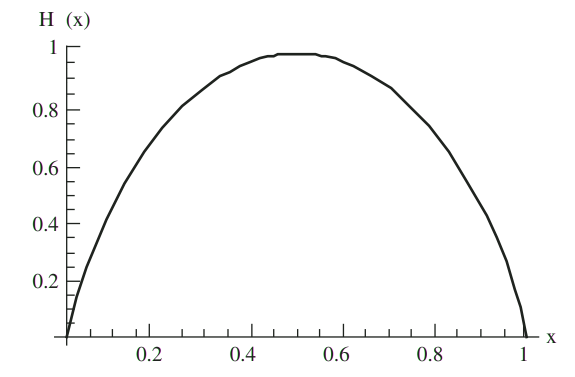
\includegraphics[width=0.5\linewidth]{../pic/3327/2.png}
    \end{center}
    If we are completely uncertain then $H(x) = 1$\\
    The general rule is that the larger the entropy, the more ignorance you have about the outcome.

    The entropy of a quantum state with density operator is given by 
    \[ S(\rho) = -Tr(\rho\log_2(\rho)) \]
    
\chapter{QUANTUM GATES}
In a classical computer, at the most fundamental level there are two basic tasks that we can use when manipulating information.\\
We can move it from one place to another, or we can do some type of basic processing on the information using a logic gate.\\
Sets of logic gates can be connected together to construct digital circuits.
\section{Classical Logic Gates}
The basic purpose of a logic gate is to manipulate or process information at the bit level in some way.
\subsection{NOT gate}	
    \begin{center}
        \begin{tabular}{|c|c|}
            \hline
             INPUT & OUTPUT \\ \hline
             0&1 \\ \hline
             1&0 \\ \hline
            \end{tabular}
    \end{center}
\subsection{OR gate}
\begin{center}
    \begin{tabular}{|c|c|c|}
        \hline
         A & B & A OR B \\ \hline
         0 & 0 & 0 \\ \hline
         0 & 1 & 1 \\ \hline
         1 & 0 & 1 \\ \hline
         1 & 1 & 1 \\ \hline
        \end{tabular}
\end{center}
\subsection{AND gate}
\begin{center}
    \begin{tabular}{|c|c|c|}
        \hline
         A & B & A AND B \\ \hline
         0 & 0 & 0 \\ \hline
         0 & 1 & 0 \\ \hline
         1 & 0 & 0 \\ \hline
         1 & 1 & 1 \\ \hline
        \end{tabular}
\end{center}
\subsection{XOR gate}
\begin{center}
    \begin{tabular}{|c|c|c|}
        \hline
         A & B & A XOR B \\ \hline
         0 & 0 & 0 \\ \hline
         0 & 1 & 1 \\ \hline
         1 & 0 & 1 \\ \hline
         1 & 1 & 0 \\ \hline
        \end{tabular}
\end{center}
\subsection{NAND gate}
\begin{center}
    \begin{tabular}{|c|c|c|}
        \hline
         A & B & A NAND B \\ \hline
         0 & 0 & 1 \\ \hline
         0 & 1 & 1 \\ \hline
         1 & 0 & 1 \\ \hline
         1 & 1 & 0 \\ \hline
        \end{tabular}
\end{center}
This gate has the interesting property of being universal. That is, all computing operations can be completed using only NAND gates.\\
In fact you can construct an entire computer using nothing but NAND gates.
\section{Single-qubit gates}
A gate can be thought of as an abstraction that represents information processing.\\
In a quantum computer the “gates” are unitary operations.
\subsection{Pauli operators}
\begin{minipage}{0.5\linewidth}
    \begin{itemize}
        \item X-GATE it is a NOT-GATE : $ \left( \begin{matrix}
         0&1   \\ 
         1&  0 \\ 
        \end{matrix}\right)$
        \item Y-GATE it is a bit flip: $ \left( \begin{matrix}
         0&-i  \\ 
         i& 0 \\ 
        \end{matrix}\right)$
        \item Z-GATE it is a phase shift: $ \left( \begin{matrix}
         1&0  \\ 
         0&  -1 \\ 
        \end{matrix}\right)$
    \end{itemize}
\end{minipage}
\begin{minipage}{0.5\linewidth}
    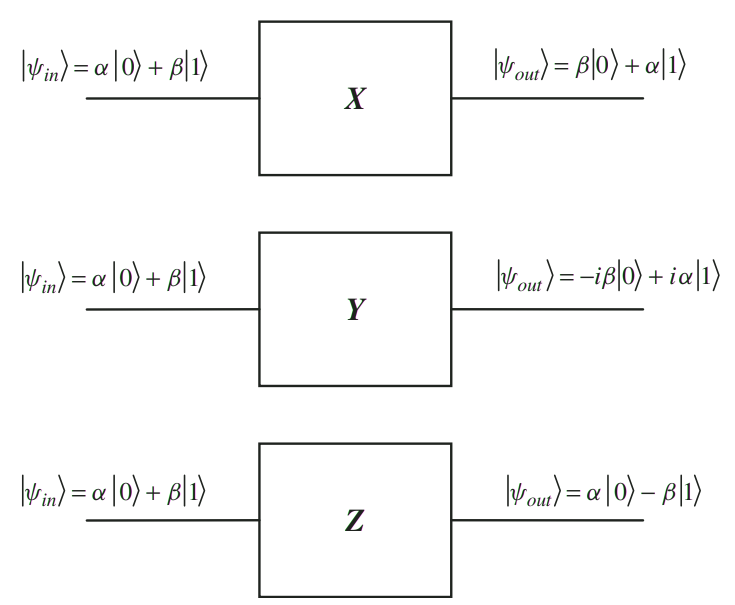
\includegraphics[width=\linewidth]{../pic/3327/3}
\end{minipage}
\subsection{Other operators}
    \begin{itemize}
        \item H-Gate (Hadamard Gate) :\\
        The Hadamard gates are used to create superposition states.\\
        $\frac{1}{\sqrt{2}} \left( \begin{matrix}
            1&1  \\ 
            1&-1 \\ 
           \end{matrix}\right) \begin{cases}
            H\ket{0} = \ket{+} \\
            H\ket{1} = \ket{-}
           \end{cases}$ , with $\ket{\pm} = \frac{\ket{0}\pm\ket{1}}{\sqrt{2}}$\\
           Two Hadamard gates in serries act to reverse the operation and give back the original input.
        \item P-Phase it is a phase shift : $\left( \begin{matrix}
            1&0  \\ 
            0&e^{i\theta} \\ 
           \end{matrix}\right) \begin{cases}
            P\ket{0} = \ket{0} \\
            P\ket{1} = e^{i\theta}\ket{1}
           \end{cases}$
    \end{itemize}
\section{The Z-Y decomposition}
We can use arbitrary unitary gate with simple geometrical interpretation in the Bloch sphere
\[ U = e^{i\alpha} R_y(...)R_z(...)R_y(...) \]
$R_y$ : rotation around the y axis.
$R_z$ : rotation around the z axis.
\section{Two-qubit gates}
We include a control bit C.\\
If C = 0, then the gate does nothing, but if C = 1, then the gate performs some specified action.
\subsection{The controlled NOT or CNOT gate.}
If the control qubit is $\ket{0}$, then nothing happens to the target qubit.\\
If the control qubit is $\ket{1}$, then the NOT or X matrix is applied to the target qubit.\\

\begin{minipage}{0.6\linewidth}
    $CNOT = \ket{0}\bra{0}\otimes I + \ket{1}\bra{1}\otimes X =  \left( \begin{matrix}
        1&  0&  0&  0  \\ 
        0&  1&  0&  0  \\ 
        0&  0&  0&  1  \\ 
        0&  0&  1&  0  \\ 
       \end{matrix}\right)$
\end{minipage}
\begin{minipage}{0.3\linewidth}
    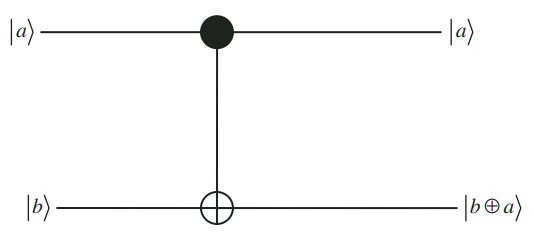
\includegraphics[width=\linewidth]{../pic/3327/4}
\end{minipage}
\subsection{The controlled-Hadamard or CH gate.}
If the control qubit is $\ket{0}$, then nothing happens to the target qubit.\\
If the control qubit is $\ket{1}$, then we apply a Hadamard gate to the target qubit.\\

\begin{minipage}{0.6\linewidth}
    $CNOT = \ket{0}\bra{0}\otimes I + \ket{1}\bra{1}\otimes X =  \left( \begin{matrix}
        1&  0&  0&  0  \\ 
        0&  1&  0&  0  \\ 
        0&  0&  \frac{1}{\sqrt{2}}&  \frac{1}{\sqrt{2}}  \\ 
        0&  0&  \frac{1}{\sqrt{2}}&  \frac{-1}{\sqrt{2}}  \\ 
       \end{matrix}\right)$
\end{minipage}
\begin{minipage}{0.3\linewidth}
    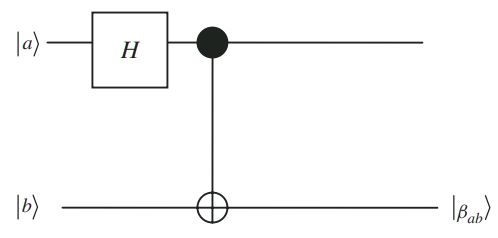
\includegraphics[width=\linewidth]{../pic/3327/5}
\end{minipage}
\section{Gate decomposition}
A large part of working with quantum circuits is decomposing an arbitrary controlled unitary operation U into a series of single-qubit operations and controlled NOT gates.
\begin{center}
    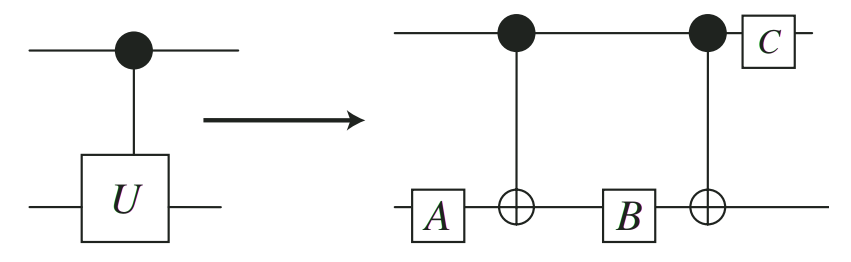
\includegraphics[width=0.3\linewidth]{../pic/3327/6.png}
\end{center}
\chapter{QUANTUM ALGORITHMS}
An algorithm is a set of instructions used to perform some well-defined task on a computer.\\
The nature of quantum systems—captured in superposition and interference of qubits—often allows a quantum system to compute in a parallel way that is not possible even, in principle, with a classical computer.
However, since measurement finds a qubit in one state or the other— frustratingly we find that if we give a quantum computer n inputs we only get n outputs.
\section{Matrix representation of serial and parallel operations}
The matrix representation of this sequence of operations is written down by multiplying the matrices in reverse order.
\[ZHP(\theta)\]
\begin{center}
    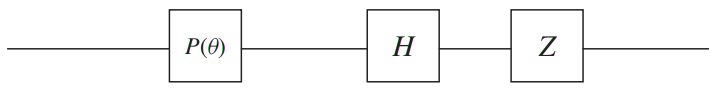
\includegraphics[width=0.5\linewidth]{../pic/3327/7.png}
\end{center}
When quantum operations are performed in parallel,we compute the tensor product.
\section{Quantum Interference}
The application of a Hadamard gate to an arbitrary qubit is an example of quantum interference.\\
There are two types of interference, positive interference in which probability amplitudes add constructively to increase or negative interference in which probability amplitudes add destructively to decrease.\\
Quantum interference allows us to gain information about a function f (x) that depends on evaluating the function at many values of x.\\
Interference allows us to deduce certain global properties of the function.
\section{Deutsch's algorithm}
consider a very simple function, one that accepts a single bit as input and produces a single bit as output.\\
For example we could have :
\begin{itemize}
    \item The identity function \\
        $f(x) = \begin{cases}
            0 \text{ if } x = 0 \\
            1 \text{ if } x = 1 \\
        \end{cases}$
    \item constant functions \\
     $f(x) = 0 , f(x) = 1$
     \item Bit flip function \\
    $f(x) = \begin{cases}
        1 \text{ if } x =0 \\
        0 \text{ if } x = 1\\
    \end{cases}$
\end{itemize}
The identity and bit flip functions are called balanced because the outputs are opposite for half the inputs.\\

Deutsch's algorithm will let us put together a state that has all of the output values of the function associated with each input value in a superposition state.\\
Then we will use quantum interference to find out if the given function is constant or balanced.\\

Deutsch's algorithm is implemented by the following steps:
\begin{itemize}
    \item Apply Hadamard gates to the input state $\ket{0}\ket{1}$ to produce a product state of two superpositions.
    \item Apply $U_f$ to that product state where $U_f$ is a unitary operation that acts on two qubits.\\
    It leaves the first qubit alone and produces the exclusive or (denoted by $\otimes$) of the second qubit with the function $f$ evaluated with the first qubit as argument.
    \[ U_f\ket{x,y} = \ket{x,y\otimes f(x)}\]
    \[ U_f\left( \frac{\ket{0} + \ket{1}}{\sqrt{2}} \right) \ket{0} = \frac{1}{\sqrt{2}}(U_f\ket{00} + U_f\ket{01}) = \frac{\ket{0,0\otimes f(0)} + \ket{1,0\otimes f(1)} }{\sqrt{2}} \]
    \item Apply a Hadamard gate to the first qubit leaving the second qubit alone.
\end{itemize}

\end{document}